\documentclass[12pt]{article}
%%---------------------------------------------------------------------
% packages
% geometry
\usepackage{geometry}
% font
\usepackage{fontspec}
\defaultfontfeatures{Mapping=tex-text}  %%如果没有它,会有一些 tex 特殊字符无法正常使用,比如连字符。
\usepackage{xunicode,xltxtra}
\usepackage[BoldFont,SlantFont,CJKnumber,CJKchecksingle]{xeCJK}  % \CJKnumber{12345}: 一万二千三百四十五
\usepackage{CJKfntef}  %%实现对汉字加点、下划线等。
\usepackage{pifont}  % \ding{}
% math
\usepackage{amsmath,amsfonts,amssymb}
% color
\usepackage{color}
\usepackage{xcolor}
\definecolor{EYE}{RGB}{199,237,204}
\definecolor{FLY}{RGB}{128,0,128}
\definecolor{ZHY}{RGB}{139,0,255}
% graphics
\usepackage[americaninductors,europeanresistors]{circuitikz}
\usepackage{tikz}
\usetikzlibrary{positioning,arrows,shadows,shapes,calc,mindmap,trees,backgrounds}  % placements=positioning
\usepackage{graphicx}  % \includegraphics[]{}
\usepackage{subfigure}  %%图形或表格并排排列
% table
\usepackage{colortbl,dcolumn}  %% 彩色表格
\usepackage{multirow}
\usepackage{multicol}
\usepackage{booktabs}
% code
\usepackage{fancyvrb}
\usepackage{listings}
% title
\usepackage{titlesec}
% head/foot
\usepackage{fancyhdr}
% ref
\usepackage{hyperref}
% pagecolor
\usepackage[pagecolor={EYE}]{pagecolor}
% tightly-packed lists
\usepackage{mdwlist}

\usepackage{styles/iplouccfg}
\usepackage{styles/zhfontcfg}
\usepackage{styles/iplouclistings}

%%---------------------------------------------------------------------
% settings
% geometry
\geometry{left=2cm,right=1cm,top=2cm,bottom=2cm}  %设置 上、左、下、右 页边距
\linespread{1.5} %行间距
% font
\setCJKmainfont{Adobe Kaiti Std}
%\setmainfont[BoldFont=Adobe Garamond Pro Bold]{Apple Garamond}  % 英文字体
%\setmainfont[BoldFont=Adobe Garamond Pro Bold,SmallCapsFont=Apple Garamond,SmallCapsFeatures={Scale=0.7}]{Apple Garamond}  %%苹果字体没有SmallCaps
\setCJKmonofont{Adobe Fangsong Std}
% graphics
\graphicspath{{figures/}}
\tikzset{
    % Define standard arrow tip
    >=stealth',
    % Define style for boxes
    punkt/.style={
           rectangle,
           rounded corners,
           draw=black, very thick,
           text width=6.5em,
           minimum height=2em,
           text centered},
    % Define arrow style
    pil/.style={
           ->,
           thick,
           shorten <=2pt,
           shorten >=2pt,},
    % Define style for FlyZhyBall
    FlyZhyBall/.style={
      circle,
      minimum size=6mm,
      inner sep=0.5pt,
      ball color=red!50!blue,
      text=white,},
    % Define style for FlyZhyRectangle
    FlyZhyRectangle/.style={
      rectangle,
      rounded corners,
      minimum size=6mm,
      ball color=red!50!blue,
      text=white,},
    % Define style for zhyfly
    zhyfly/.style={
      rectangle,
      rounded corners,
      minimum size=6mm,
      ball color=red!25!blue,
      text=white,},
    % Define style for new rectangle
    nrectangle/.style={
      rectangle,
      draw=#1!50,
      fill=#1!20,
      minimum size=5mm,
      inner sep=0.1pt,}
}
\ctikzset{
  bipoles/length=.8cm
}
% code
\lstnewenvironment{VHDLcode}[1][]{%
  \lstset{
    basicstyle=\footnotesize\ttfamily\color{black},%
    columns=flexible,%
    framexleftmargin=.7mm,frame=shadowbox,%
    rulesepcolor=\color{blue},%
%    frame=single,%
    backgroundcolor=\color{yellow!20},%
    xleftmargin=1.2\fboxsep,%
    xrightmargin=.7\fboxsep,%
    numbers=left,numberstyle=\tiny\color{blue},%
    numberblanklines=false,numbersep=7pt,%
    language=VHDL%
    }\lstset{#1}}{}
\lstnewenvironment{VHDLmiddle}[1][]{%
  \lstset{
    basicstyle=\scriptsize\ttfamily\color{black},%
    columns=flexible,%
    framexleftmargin=.7mm,frame=shadowbox,%
    rulesepcolor=\color{blue},%
%    frame=single,%
    backgroundcolor=\color{yellow!20},%
    xleftmargin=1.2\fboxsep,%
    xrightmargin=.7\fboxsep,%
    numbers=left,numberstyle=\tiny\color{blue},%
    numberblanklines=false,numbersep=7pt,%
    language=VHDL%
    }\lstset{#1}}{}
\lstnewenvironment{VHDLsmall}[1][]{%
  \lstset{
    basicstyle=\tiny\ttfamily\color{black},%
    columns=flexible,%
    framexleftmargin=.7mm,frame=shadowbox,%
    rulesepcolor=\color{blue},%
%    frame=single,%
    backgroundcolor=\color{yellow!20},%
    xleftmargin=1.2\fboxsep,%
    xrightmargin=.7\fboxsep,%
    numbers=left,numberstyle=\tiny\color{blue},%
    numberblanklines=false,numbersep=7pt,%
    language=VHDL%
    }\lstset{#1}}{}
% pdf
\hypersetup{pdfpagemode=FullScreen,%
            pdfauthor={Haiyong Zheng},%
            pdftitle={Title},%
            CJKbookmarks=true,%
            bookmarksnumbered=true,%
            bookmarksopen=false,%
            plainpages=false,%
            colorlinks=true,%
            citecolor=green,%
            filecolor=magenta,%
            linkcolor=cyan,%red(default)
            urlcolor=cyan}
% section
%http://tex.stackexchange.com/questions/34288/how-to-place-a-shaded-box-around-a-section-label-and-name
\newcommand\titlebar{%
\tikz[baseline,trim left=3.1cm,trim right=3cm] {
    \fill [cyan!25] (2.5cm,-1ex) rectangle (\textwidth+3.1cm,2.5ex);
    \node [
        fill=cyan!60!white,
        anchor= base east,
        rounded rectangle,
        minimum height=3.5ex] at (3cm,0) {
        \textbf{\thesection.}
    };
}%
}
\titleformat{\section}{\Large\bf\color{blue}}{\titlebar}{0.1cm}{}
% head/foot
\setlength{\headheight}{15pt}
\pagestyle{fancy}
\fancyhf{}
%\lhead{\color{black!50!green}2014年秋季学期}
\chead{\color{black!50!green}关于超像素分割方法的总结}
%\rhead{\color{black!50!green}通信电子电路}
\lfoot{\color{blue!50!green}朱亚菲}
\cfoot{\color{blue!50!green}\href{http://vision.ouc.edu.cn/~zhenghaiyong}{CVBIOUC}}
\rfoot{\color{blue!50!green}$\cdot$\ \thepage\ $\cdot$}
\renewcommand{\headrulewidth}{0.4pt}
\renewcommand{\footrulewidth}{0.4pt}

%%---------------------------------------------------------------------
\begin{document}
%%---------------------------------------------------------------------
%%---------------------------------------------------------------------
% \titlepage
\title{\vspace{-2em}关于超像素分割方法的总结\vspace{-0.7em}}
\author{朱亚菲}
\date{\vspace{-0.7em}2015年1月\vspace{-0.7em}}
%%---------------------------------------------------------------------
\maketitle\thispagestyle{fancy}
%%---------------------------------------------------------------------
\maketitle
\tableofcontents 


\section{引言}

图像分割是指按照一定的相似性准则将图像划分为具有特殊语义的不同区域,其研究最早可以追溯至20世纪60年代,已历经几十年的发展,图像分割作为计算机视觉领域的基本问题,是图像理解的重要组成部分。与此同时,它在图像处理、模式识别和人工智能等多个领域也扮演了关键的角色。

目前对图像的处理大多以像素为单位,用二维矩阵来表示一幅图像,并未考虑像素之间的空间组织关系,这使得算法处理效率过低。2003年,Ren等人~\cite{1}最早提出了超像素这一概念,所谓超像素,是指具有相似纹理、颜色、亮度等特征的相邻像素构成的图像块。它利用像素之间特征的相似程度将像素分组,可以获取图像的冗余信息,在很大程度上降低了后续图像处理任务的复杂度。

超像素生成算法大致可分为基于图论的方法、基于梯度上升的方法两类~\cite{4} 。

\section{基于图论的超像素分割方法}

基于图论\footnote{图论的产生源于18世纪的著名古典数学问题之---哥尼斯堡七桥问题,问题提出后,很多人对此很感兴趣,纷纷进行试验,但在相当长的时间里,始终未能解决。1736年29岁的欧拉向圣彼得堡科学院递交了《哥尼斯堡的七座桥》的论文,在解决问题的同时,开创了数学的一个新的分支---图论与几何拓扑。}的超像素分割方法将


\subsection{Graph-based segmentation}

Felzenszwalb and Huttenlocher~\cite{8}, 
http://cs.brown.edu/~pff/segment/

\section{基于梯度上升的超像素分割方法}

梯度上升方法是从一个粗糙的像素的初始聚类开始,通过不断的迭代来优化聚类簇,直至满足收敛准则以形成超像素。以下几种方法都采用了聚类的基本思想,但各自具体方法不同,也有不同的优缺点。

\subsection{Mean-shift算法}

关键词:核函数、Mean Shift向量、

\subsubsection{原理}

Mean shift的含义随着理论的发展在不断发生着变化,其最初含义是偏移的均值向量,最早是由Fukunaga和Hostetler~\cite{6}在1975年的一篇关于非参数概率密度函数梯度的估计的文章中提出来的,其中Mean shift只是一个简单的表示向量的名词。

直到1995年,Cheng~\cite{7}的论文发表才引起人们的研究兴趣,掀起了研究和应用Mean Shift算法的热潮。近年来,Mean Shift算法已广泛应用于计算机视觉与模式识别领域,例如目标跟踪、图像分割、模式识别与聚类分析、滤波、信息融合、特征空间分析等。

Comaniciu等人~\cite{5}于2002年提出了一种无参数的、基于核密度估计的迭代算法。其基本思想如下:

1)给定在$d$维空间上的$n$个数据点$x_i, i = 1, \ldots, n$,

2)

3)

\subsubsection{应用}

1. 梯度聚类算法

如图\ref{fig:1}

2. 

1)聚类,数据集${x_i, i = 1, \ldots, n}$中的每一个点都可以作为初始点,分别执行Mean Shift算法,收敛到同一个点算作一类;

\subsection{Turbopixel}

\subsection{SLIC算法}

SLIC是Simple Linear Iterative Clustering的缩写,最早由Achanta~\cite{2}于2010年6月在洛桑联邦理工学院的一次技术报告中提出。2012年经整理、完善后发表在TPAMI上~\cite{3}。其中“Linear”体现在算法复杂度$O(N)$与图像中像素个数$N$是线性关系,“Clustering"是采用k-均值聚类。

SLIC是一种使用简单和易于理解的方法,是对传统的k-均值超像素分割方法的改进。两者之间主要有以下两点区别:

1. SLIC优化了距离计算的数目,传统的k-均值方法中每个聚类中心的搜索范围是整幅图像,要计算该聚类中心与图像中所有像素点之间的距离,而SLIC算法只在与预设的超像素尺寸成比例的一个区域内搜索,见图\ref{fig:2}。

2. SLIC算法在计算聚类中心与像素点之间的距离时同时结合了颜色和空间位置两方面的信息来表征其相似度,这样可以起到控制超像素尺寸和紧密度的作用。

默认情况下,该算法只有一个参数$k$,即所需生成的近似同样大小的超像素的个数。具体步骤为:

a)初始化聚类中心。假设一幅彩色图像有$N$个像素点,预分割为$k$个相同尺寸的超像素,那么首先要将该彩色图像转换为CIELAB颜色空间和XY坐标下的5维特征向量,然后将图像均分为$k$个网格,网格边长为$S=\sqrt{N/k}$,k个初始聚类中心$C_i=[l_i, a_i, b_i, x_i, y_i]^T$为每个网格内色阶值最低的像素。对图像中的每一个像素点,令其与最近的聚类中心的距离$d(i)$的初始值为$\infty$。

b)相似度衡量。对于每个聚类中心,逐一计算其$2S \times 2S$邻域内(如图\ref{fig:2})各像素$i$与该类中心点的距离$D$,若$D<d(i)$,则$i$暂时归为该类,并且将$d(i)$赋值为$D$,其中
\begin{align}
d_c & =  \sqrt{(l_j-l_i)^2+(a_j-a_i)^2+(b_j-b_i)^2}\\
d_s & =  \sqrt{(x_j-x_i)^2+(y_j-y_i)^2}\\
D & =  \sqrt{d_c^2+\left(\frac{d_s}{S}\right)^2m^2}
\end{align}

c)确定新的聚类中心。当每个像素都被归类到其最近的聚类中心后,新的聚类中心为该类中所有像素的$[l, a, b, x, y]^T$向量的平均值。为了避免聚类中心落在边界上,以及对后续的聚类过程造成干扰,需要将聚类中心在以$3\times3$的邻域内打乱,将聚类中心移到邻域内梯度最小的地方(图像灰度值变化最缓慢的地方)。计算残差$E$(新的聚类中心与之前聚类中心的$L1$范数)。

d)重复b)和c)直至最后收敛($E\le threshold$)。

\begin{figure}[!ht]
\centering
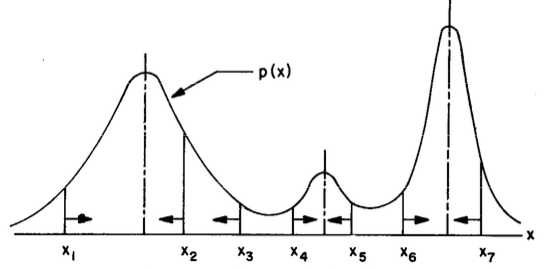
\includegraphics[width=0.6\textwidth]{1.png}
\caption{梯度模式聚类}
\label{fig:1}
\end{figure} 

\begin{figure}[!ht]
\centering
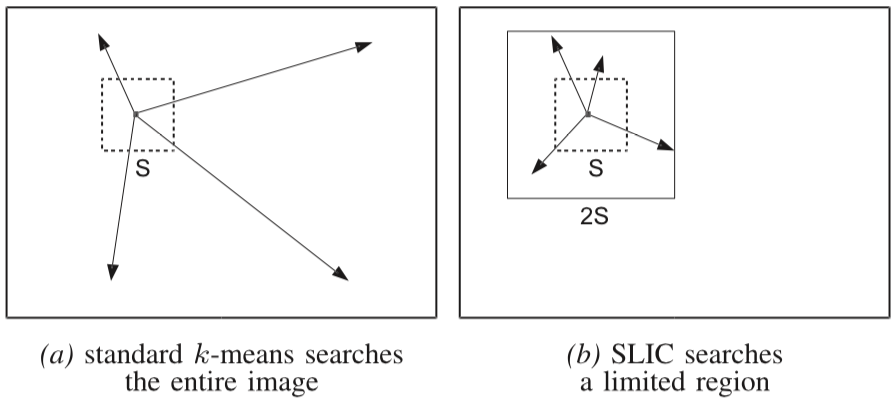
\includegraphics[width=0.7\textwidth]{2.png}
\caption{传统的k-均值方法与SLIC算法搜索区域的区别}
\label{fig:2}
\end{figure} 

\section{实验效果分析}



% references
\bibliographystyle{plain}

\bibliography{template} %参考文献


%%---------------------------------------------------------------------
\end{document}
